\subsection{Unfolding}
The effects of imperfect detector resolution can in general have an non-negligible impact on the shape of the distribution of the measured observables. For this reason, in case of the differential cross sections measurements, a procedure to correct for the detection efficiencies and
 resolution effects is applied. Throughout this document, this procedure will be referred to as
 the unfolding procedure, and the unfolded differential distributions will be referred to as distributions at the fiducial level. 
 Currently adopted procedure is ``bin-by-bin unfolding''. This procedure for the unfolding of the detector effects from the observed distributions is the same as in Refs.~\cite{CMSH4lFiducial8TeV}~and~\cite{CMSHggFiducial8TeV}. 
The finite efficiencies and resolution effects are encoded in a detector response matrix which describes how events migrate from a given observable bin at the fiducial level to a given bin at the reconstruction level. This matrix is diagonally dominant, with sizeable off-diagonal elements for observables involving jets.
 It is aimed we would also perform matrix inversion method as a validation tool for preceding method.

Examples of the efficiency matrices for gluon fusion and VBF production can be seen in Fig.~\ref{fig:eff2d}. The matrices for the $\pt_{\rm H}$ and N(jets) observables are shown.

\begin{figure}[!h]
       \centering
       \includegraphics[width=0.32\linewidth]{Figures/results/fiducial/2016/eff2d_ggH_powheg_JHUgen_125_pT4l_2e2mu.pdf}
       \includegraphics[width=0.32\linewidth]{Figures/results/fiducial/2017/eff2d_ggH_powheg_JHUgen_125_pT4l_2e2mu.pdf}
       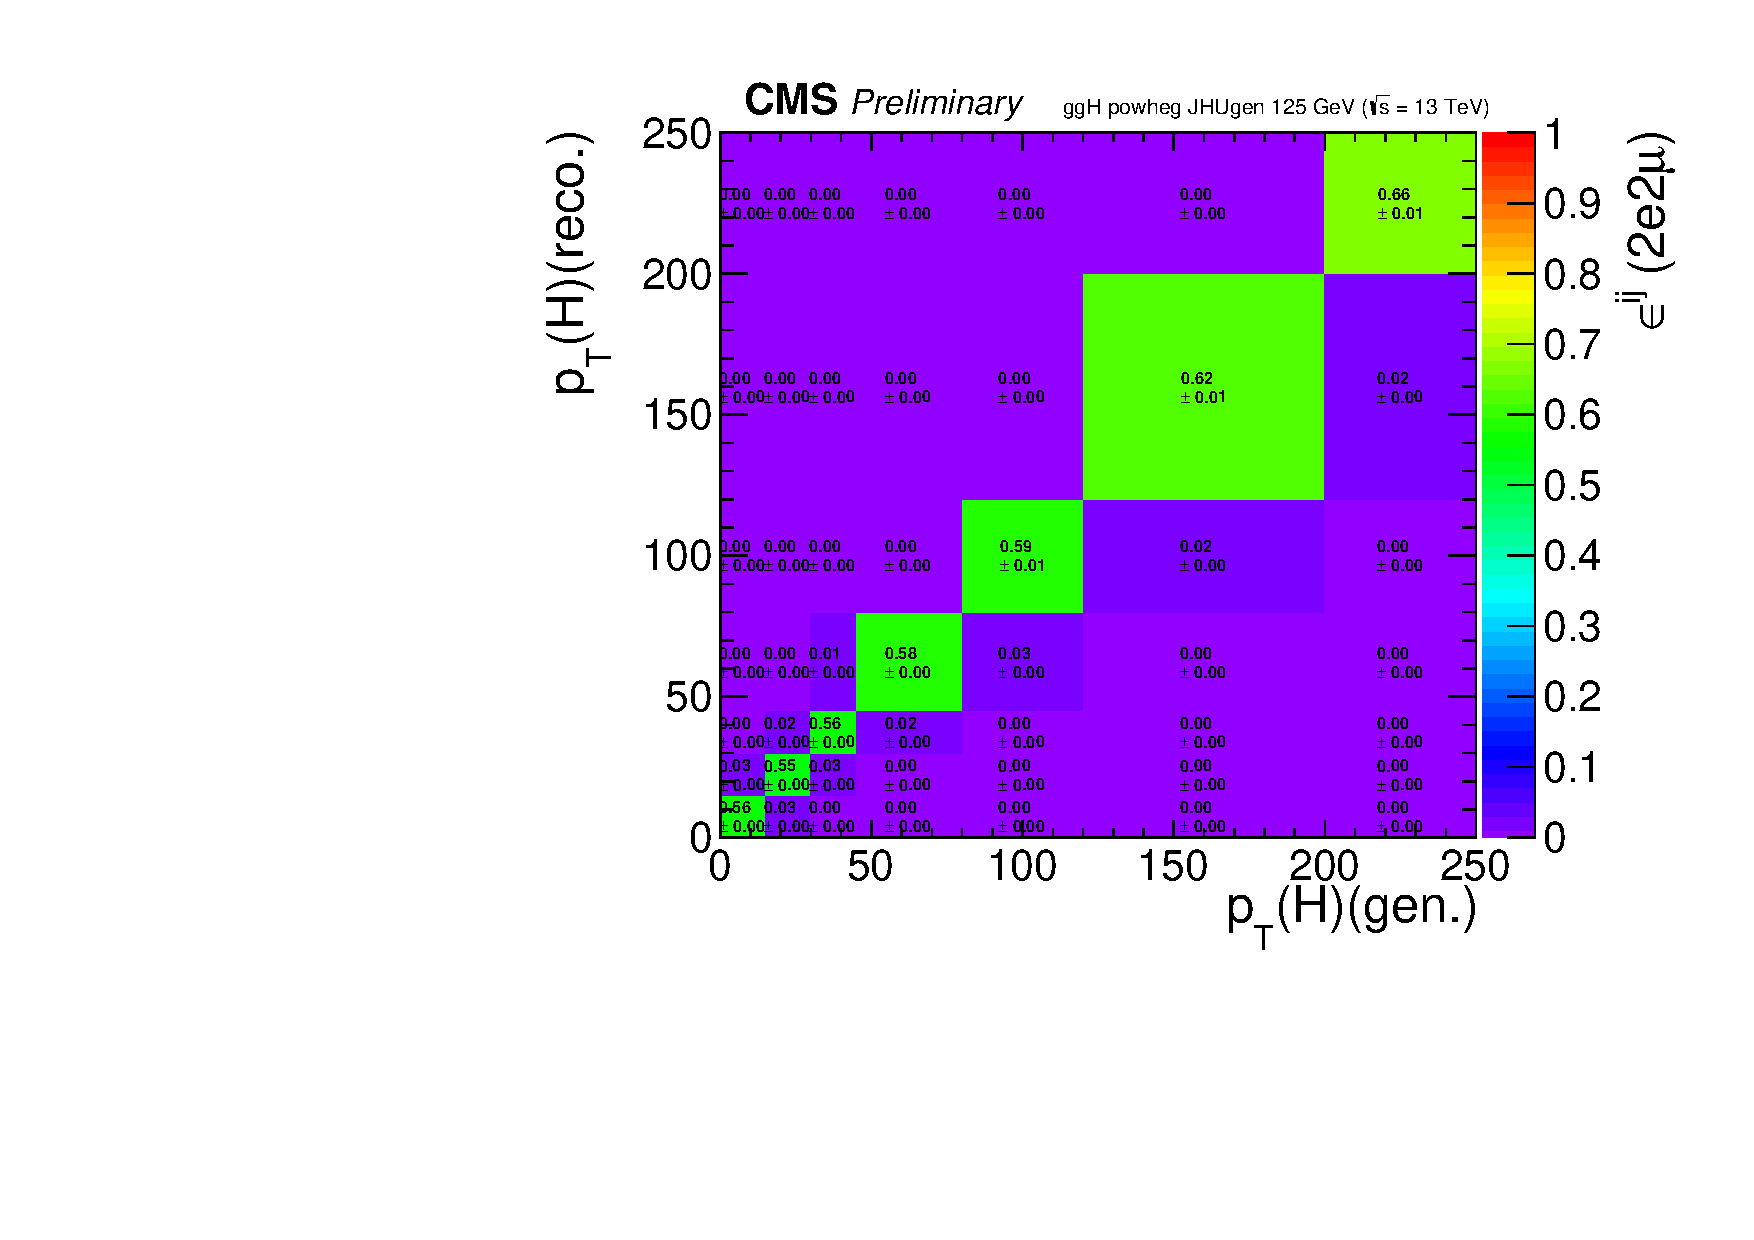
\includegraphics[width=0.32\linewidth]{Figures/results/fiducial/2018/eff2d_ggH_powheg_JHUgen_125_pT4l_2e2mu.pdf} \\
       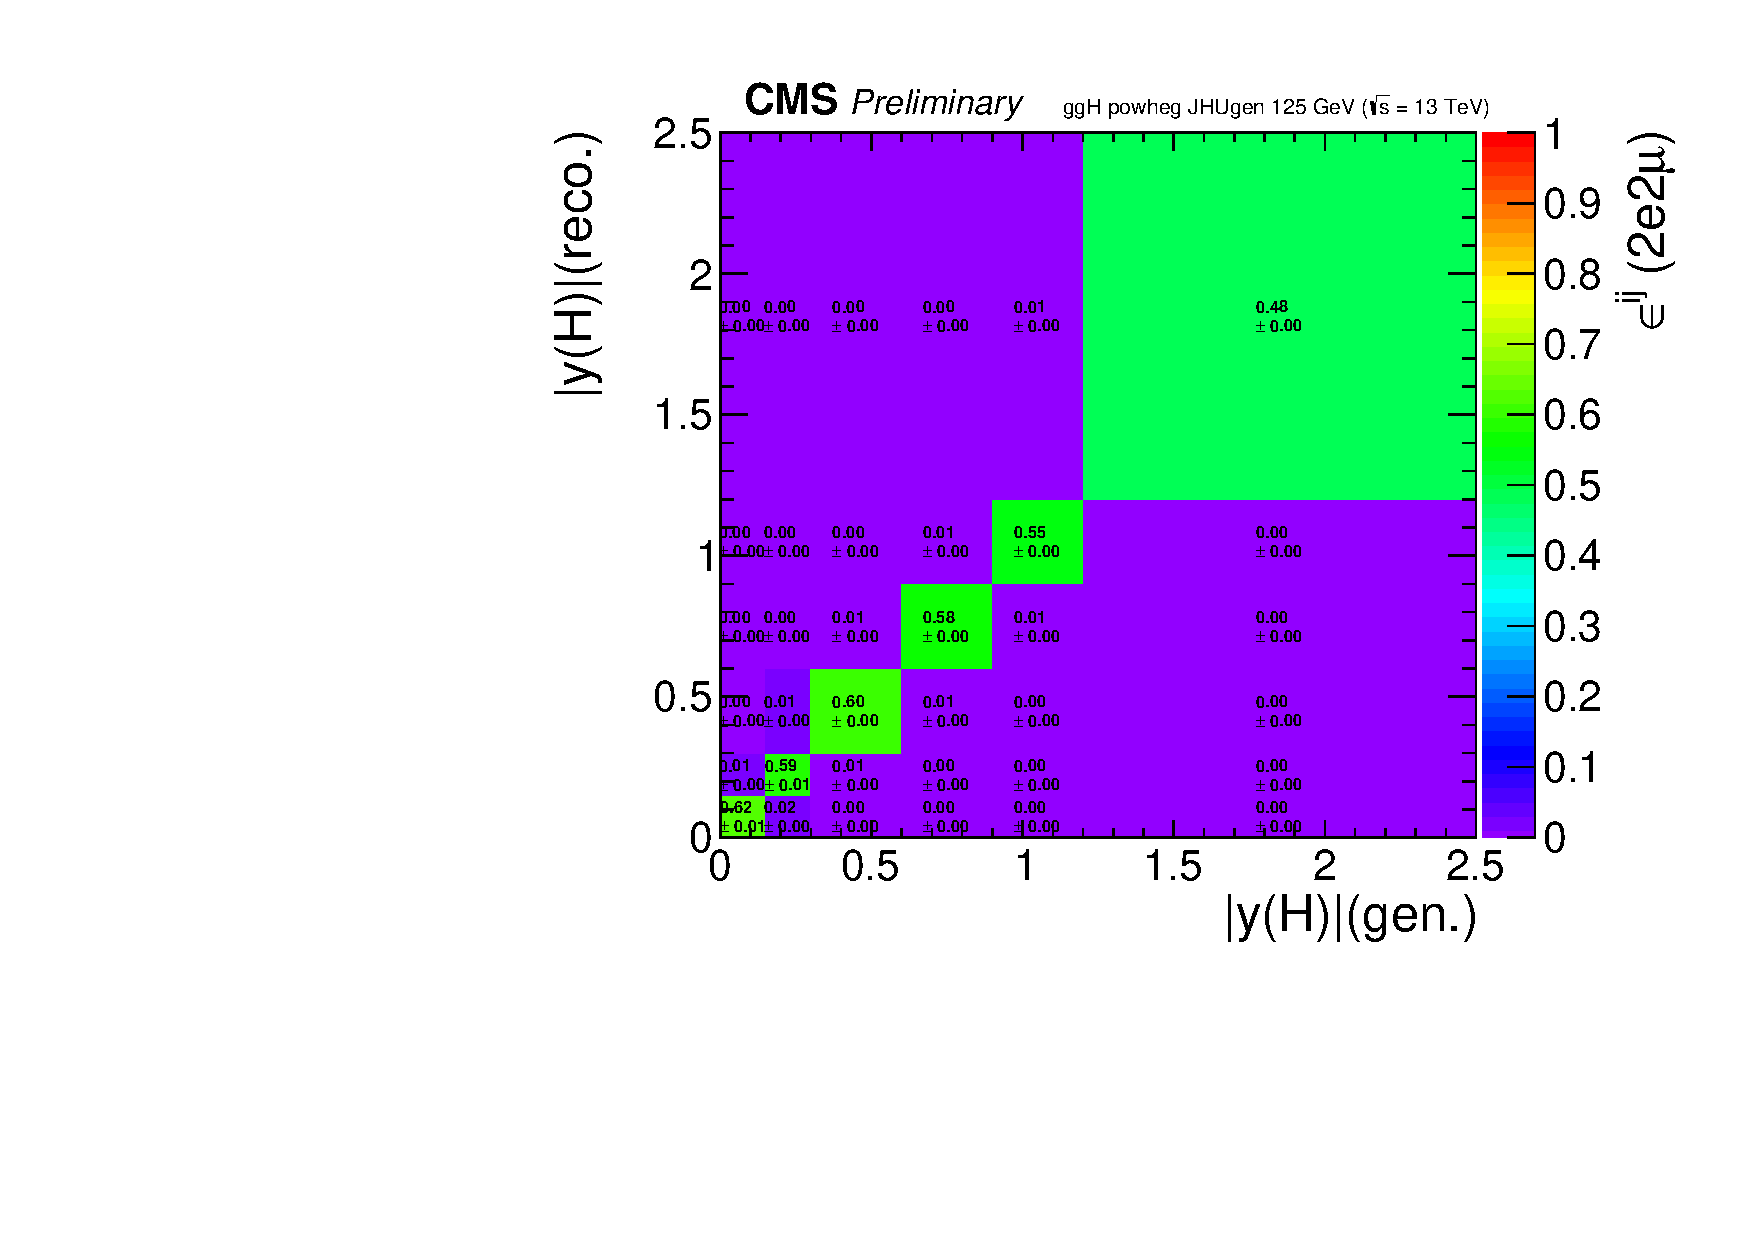
\includegraphics[width=0.32\linewidth]{Figures/results/fiducial/2016/eff2d_ggH_powheg_JHUgen_125_rapidity4l_2e2mu.pdf}
       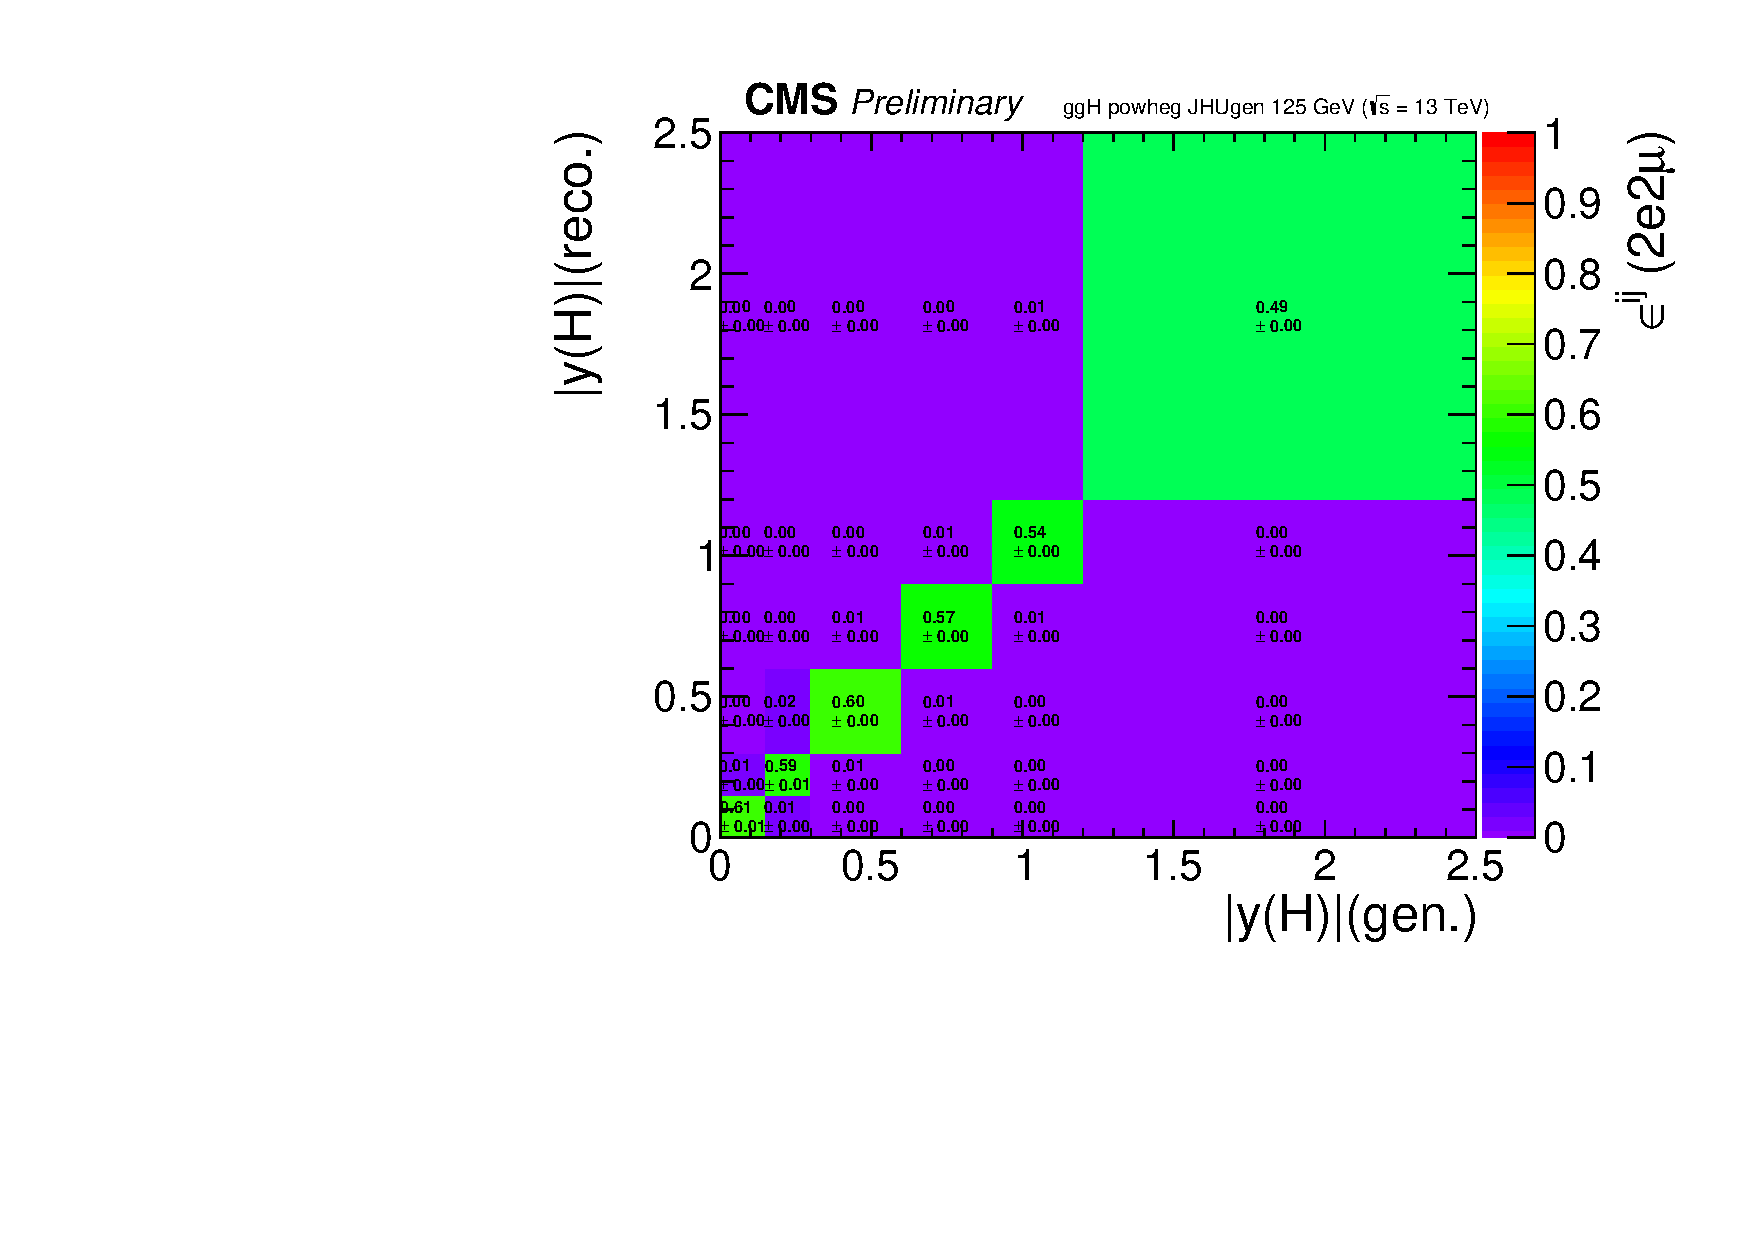
\includegraphics[width=0.32\linewidth]{Figures/results/fiducial/2017/eff2d_ggH_powheg_JHUgen_125_rapidity4l_2e2mu.pdf}
       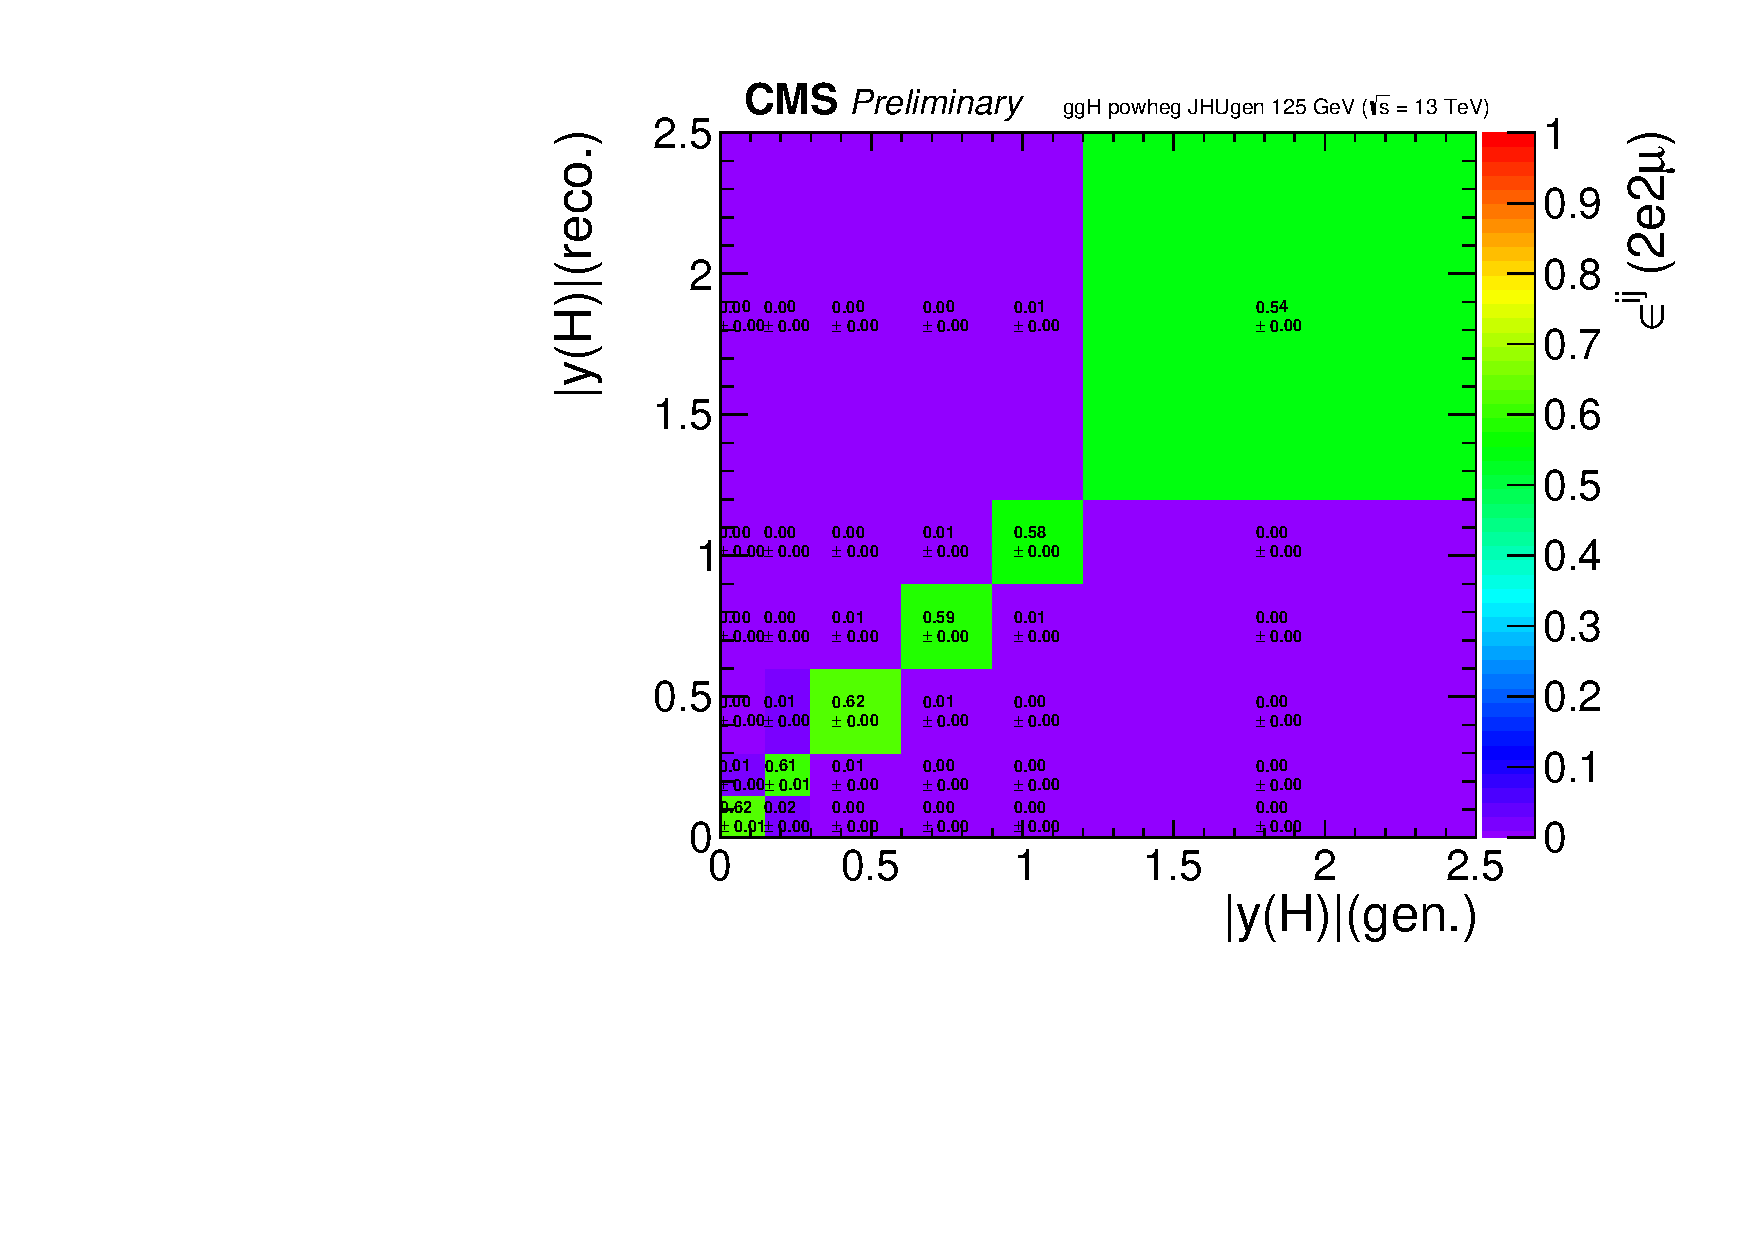
\includegraphics[width=0.32\linewidth]{Figures/results/fiducial/2018/eff2d_ggH_powheg_JHUgen_125_rapidity4l_2e2mu.pdf} \\
       \includegraphics[width=0.32\linewidth]{Figures/results/fiducial/2016/eff2d_ggH_powheg_JHUgen_125_njets_pt30_eta2p5_2e2mu.pdf}
       \includegraphics[width=0.32\linewidth]{Figures/results/fiducial/2017/eff2d_ggH_powheg_JHUgen_125_njets_pt30_eta2p5_2e2mu.pdf}
       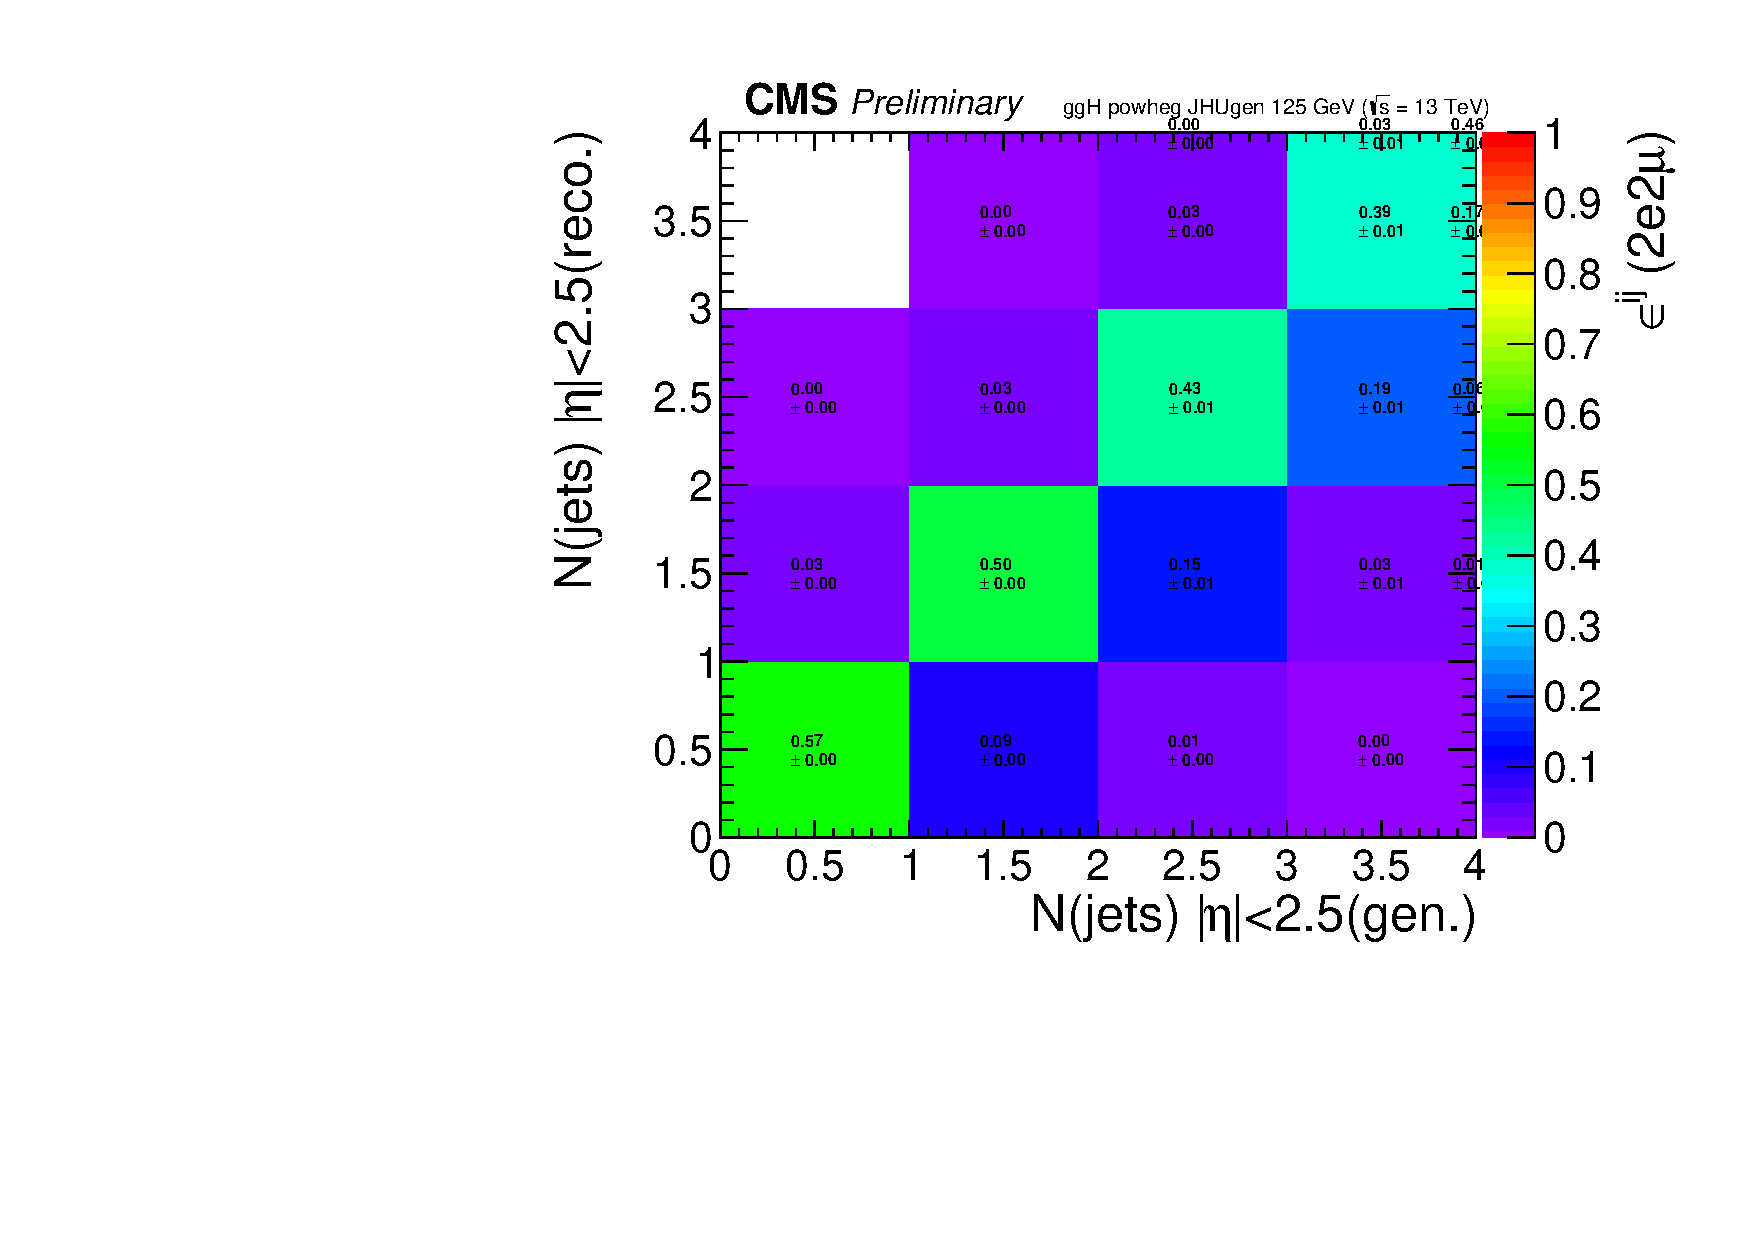
\includegraphics[width=0.32\linewidth]{Figures/results/fiducial/2018/eff2d_ggH_powheg_JHUgen_125_njets_pt30_eta2p5_2e2mu.pdf}

       \caption{Efficiency matrices for the $\pt_{\rm H}$ (top) and $y{\rm H}$ (middle) and N(jets) (bottom) observables for gluon fusion production
	       modes in the $2e2\mu$ final state in 2016 (left) 2017 (middle) and 2018 (right) (TBU). \label{fig:eff2d}}
\end{figure}
%The reconstruction level selection, fiducial volume definition,
%statistical procedure, and their model dependence will be described the subsequent sections.

